\chapter{Diseño e implementación} % Main chapter title

\label{Chapter3} % Change X to a consecutive number; for referencing this chapter elsewhere, use \ref{ChapterX}

\definecolor{mygreen}{rgb}{0,0.6,0}
\definecolor{mygray}{rgb}{0.5,0.5,0.5}
\definecolor{mymauve}{rgb}{0.58,0,0.82}

%%%%%%%%%%%%%%%%%%%%%%%%%%%%%%%%%%%%%%%%%%%%%%%%%%%%%%%%%%%%%%%%%%%%%%%%%%%%%
% parámetros para configurar el formato del código en los entornos lstlisting
%%%%%%%%%%%%%%%%%%%%%%%%%%%%%%%%%%%%%%%%%%%%%%%%%%%%%%%%%%%%%%%%%%%%%%%%%%%%%
\lstset{ %
  backgroundcolor=\color{white},   % choose the background color; you must add \usepackage{color} or \usepackage{xcolor}
  basicstyle=\footnotesize,        % the size of the fonts that are used for the code
  breakatwhitespace=false,         % sets if automatic breaks should only happen at whitespace
  breaklines=true,                 % sets automatic line breaking
  captionpos=b,                    % sets the caption-position to bottom
  commentstyle=\color{mygreen},    % comment style
  deletekeywords={...},            % if you want to delete keywords from the given language
  %escapeinside={\%*}{*)},          % if you want to add LaTeX within your code
  %extendedchars=true,              % lets you use non-ASCII characters; for 8-bits encodings only, does not work with UTF-8
  %frame=single,	                % adds a frame around the code
  keepspaces=true,                 % keeps spaces in text, useful for keeping indentation of code (possibly needs columns=flexible)
  keywordstyle=\color{blue},       % keyword style
  language=[ANSI]C,                % the language of the code
  %otherkeywords={*,...},           % if you want to add more keywords to the set
  numbers=left,                    % where to put the line-numbers; possible values are (none, left, right)
  numbersep=5pt,                   % how far the line-numbers are from the code
  numberstyle=\tiny\color{mygray}, % the style that is used for the line-numbers
  rulecolor=\color{black},         % if not set, the frame-color may be changed on line-breaks within not-black text (e.g. comments (green here))
  showspaces=false,                % show spaces everywhere adding particular underscores; it overrides 'showstringspaces'
  showstringspaces=false,          % underline spaces within strings only
  showtabs=false,                  % show tabs within strings adding particular underscores
  stepnumber=1,                    % the step between two line-numbers. If it's 1, each line will be numbered
  stringstyle=\color{mymauve},     % string literal style
  tabsize=2,	                   % sets default tabsize to 2 spaces
  title=\lstname,                  % show the filename of files included with \lstinputlisting; also try caption instead of title
  morecomment=[s]{/*}{*/}
}


%----------------------------------------------------------------------------------------
%	SECTION 1
%----------------------------------------------------------------------------------------
\section{Arquitectura general del sistema}
\label{sec:arquitecturagral}

\subsection{Funcionamiento}
\label{subsec:funcionamiento}
Como se puede observar en la figura \ref{fig:diagramafunciones}, el sistema está compuesto por nodos los cuales se utilizan para la lectura de tarjetas RFID asignadas a los repuestos de los clientes. Los datos se transmiten en una red lan local, se procesan y almacenan en un servidor con base de datos y son consultados desde la aplicación web en las terminales (\textit{PC} o \textit{smartphone}).

\begin{figure}[ht]
	\centering
	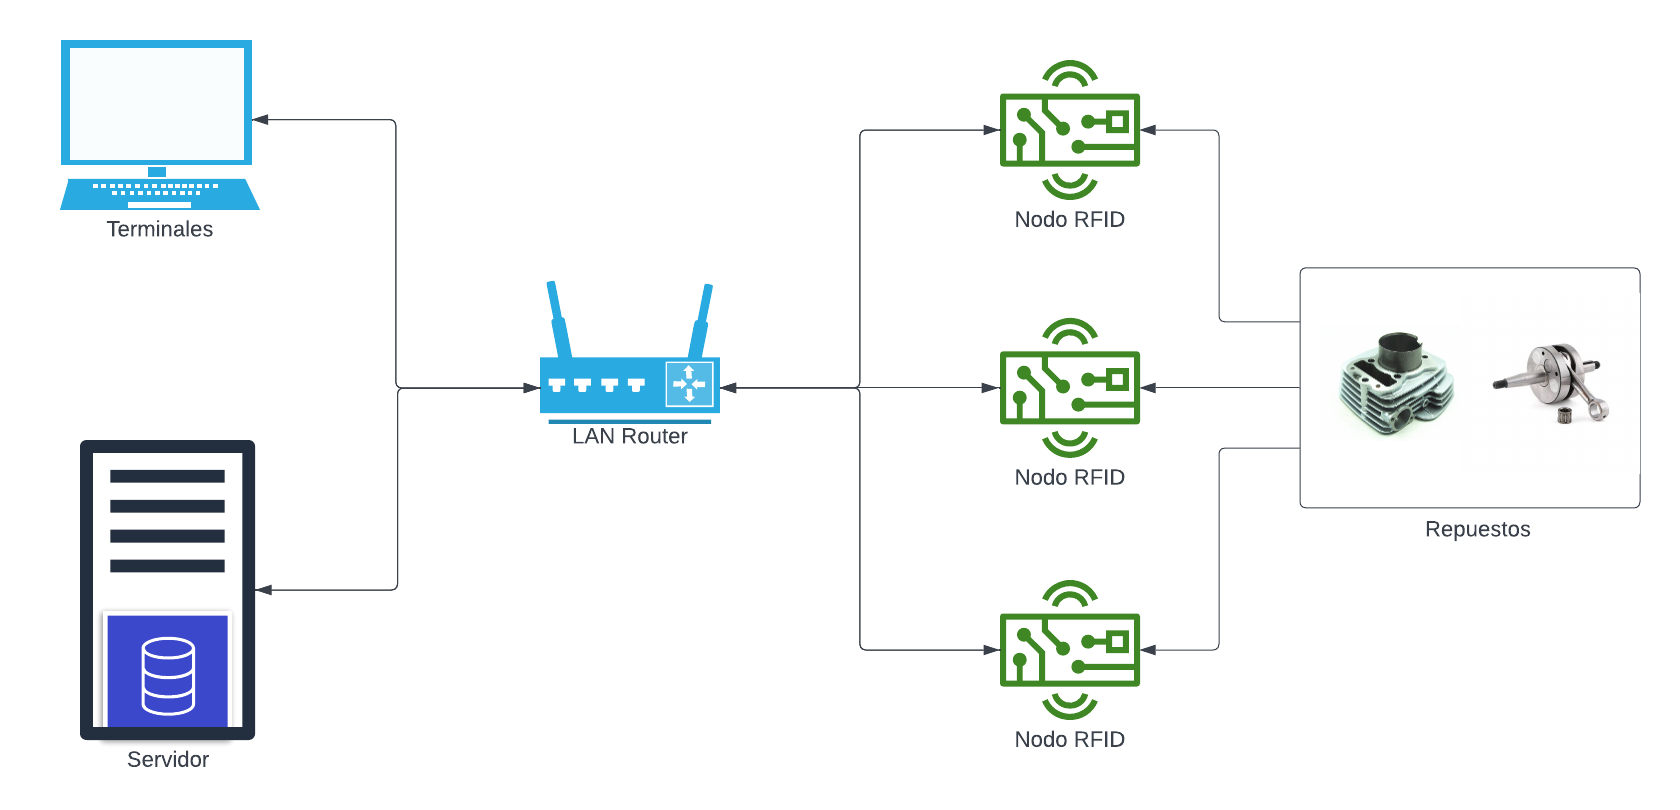
\includegraphics[scale=.20]{./Figures/diagramafunciones.png}
	\caption{Diagrama de funciones generales.}
	\label{fig:diagramafunciones}
\end{figure}

\subsection{Diagrama de bloques}
\label{subsec:diagramabloques}
En la figura \ref{fig:diagramabloques} se representa el patrón de modelo conceptual empleado y las tecnologías que se utilizan en cada capa. Se implementó un modelo de 4 capas: 

\begin{itemize}
\item Capa de percepción.
\item Capa de transporte.
\item Capa de procesamiento.
\item Capa de aplicación.
\end{itemize}


\begin{figure}[ht]
	\centering
	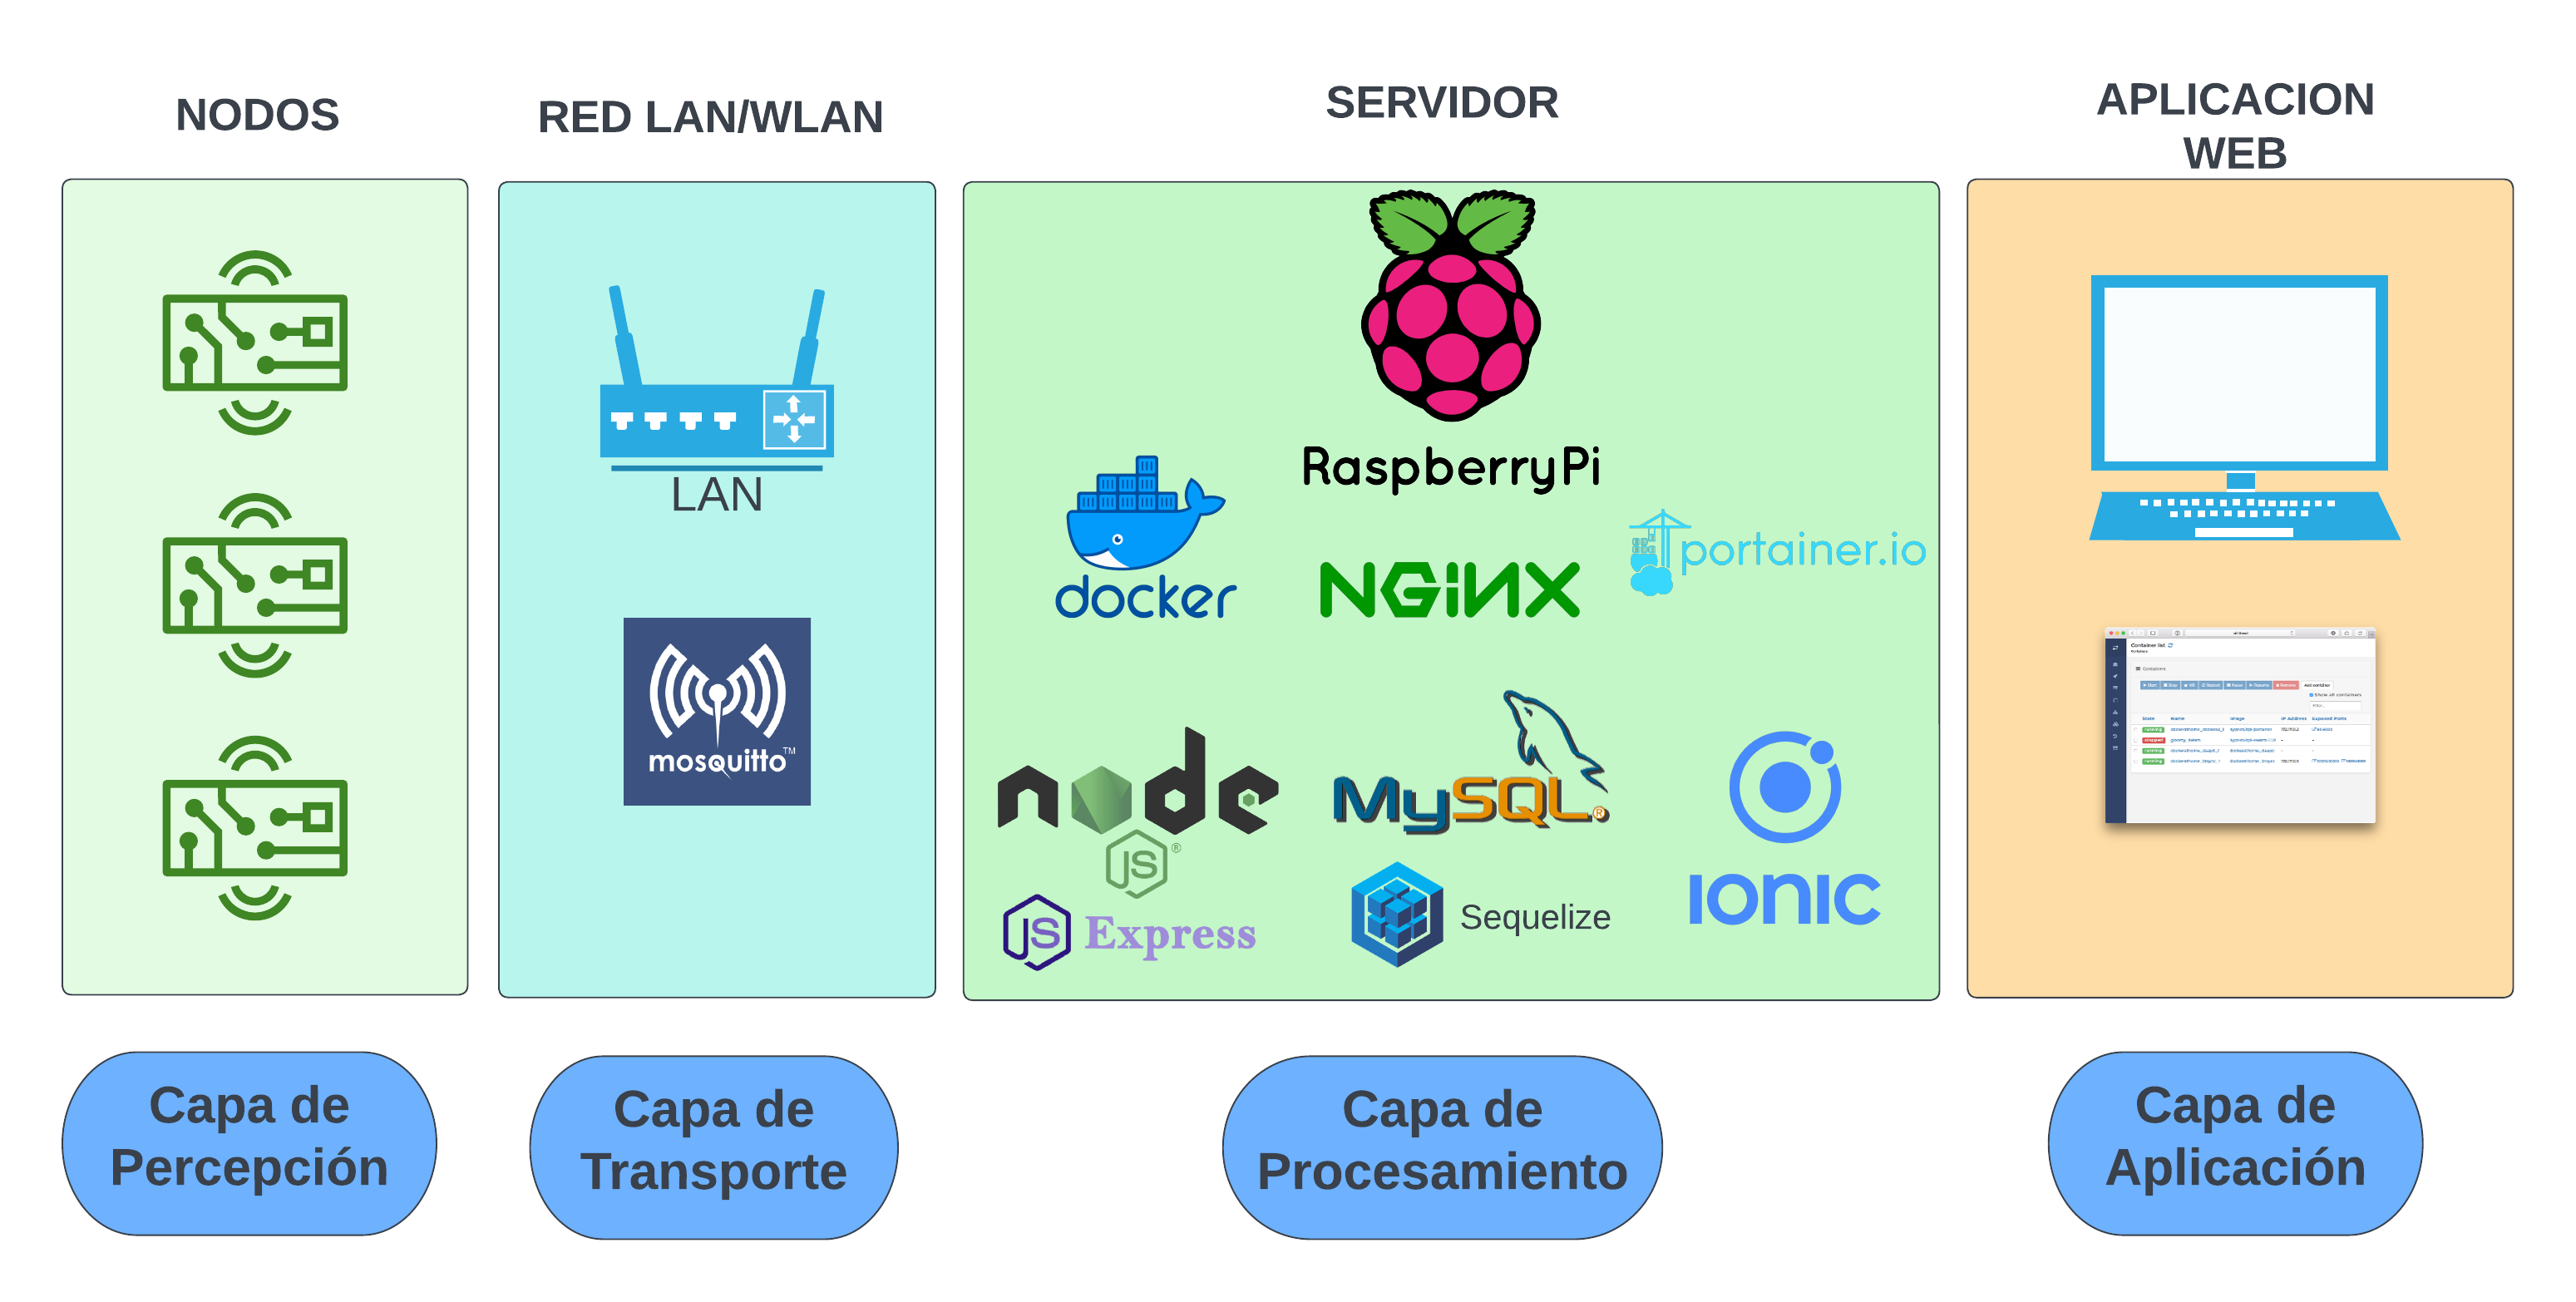
\includegraphics[scale=.25]{./Figures/diagramabloques.png}
	\caption{Diagrama de bloques y tecnologías del sistema.}
	\label{fig:diagramabloques}
\end{figure}


En la capa de percepción se utilizan los nodos esp32 con lector RFID con los cuales se realiza la lectura de las tarjetas correspondientes. Una vez realizada la lectura, los datos son enviados por medio del protocolo MQTT y a traves de la red lan en la capa de transporte. 

La capa de transporte es la encargada de transmitir los mensajes por medio de los protocolos MQTT y HTTP. El broker \textit{Eclipse Mosquitto} distribuye los mensajes publicados a los subscriptores para su procesamiento.

En la capa de procesamiento se realiza la lógica del backend, la base de datos y el frontend. Se implementó un servidor central en una Raspberry Pi 4 con todos los servicios. Cada uno de los servicios está desarrollado de manera individual y fue montado en su propio contenedor de Docker. Todos los contenedores se despliegan utilizando Docker Compose.

Por último, la capa de aplicación otorga el acceso web desarrollado en el framework \textit{Ionic} para el ingreso, registro, administración y egreso de las ordenes de trabajo y también se utiliza el portal de administración de \textit{Portainer} para el monitoreo completo de Docker y del servidor.


\section{Flujo general del sistema}
\label{sec:flujogeneral}
En esta sección se explica el flujo total de las funciones del sistema desde que el usuario ingresa una nueva orden de trabajo hasta que el producto es retirado por el cliente.

Las comunicaciones y el envío de datos entre los distintos módulos del sistema se realizan en los protocolos HTTP, MQTT y MySQL. Se detallará en cada caso el protocolo utilizado.

\subsection{Ingreso de repuesto}
\label{subsec:ingresorepuesto}
En la figura \ref{fig:flujoingreso} se puede observar todos los módulos del sistema, el flujo de datos y el protocolo utilizado cuando un usuario carga una nueva orden de trabajo en el sistema.

\begin{figure}[ht]
	\centering
	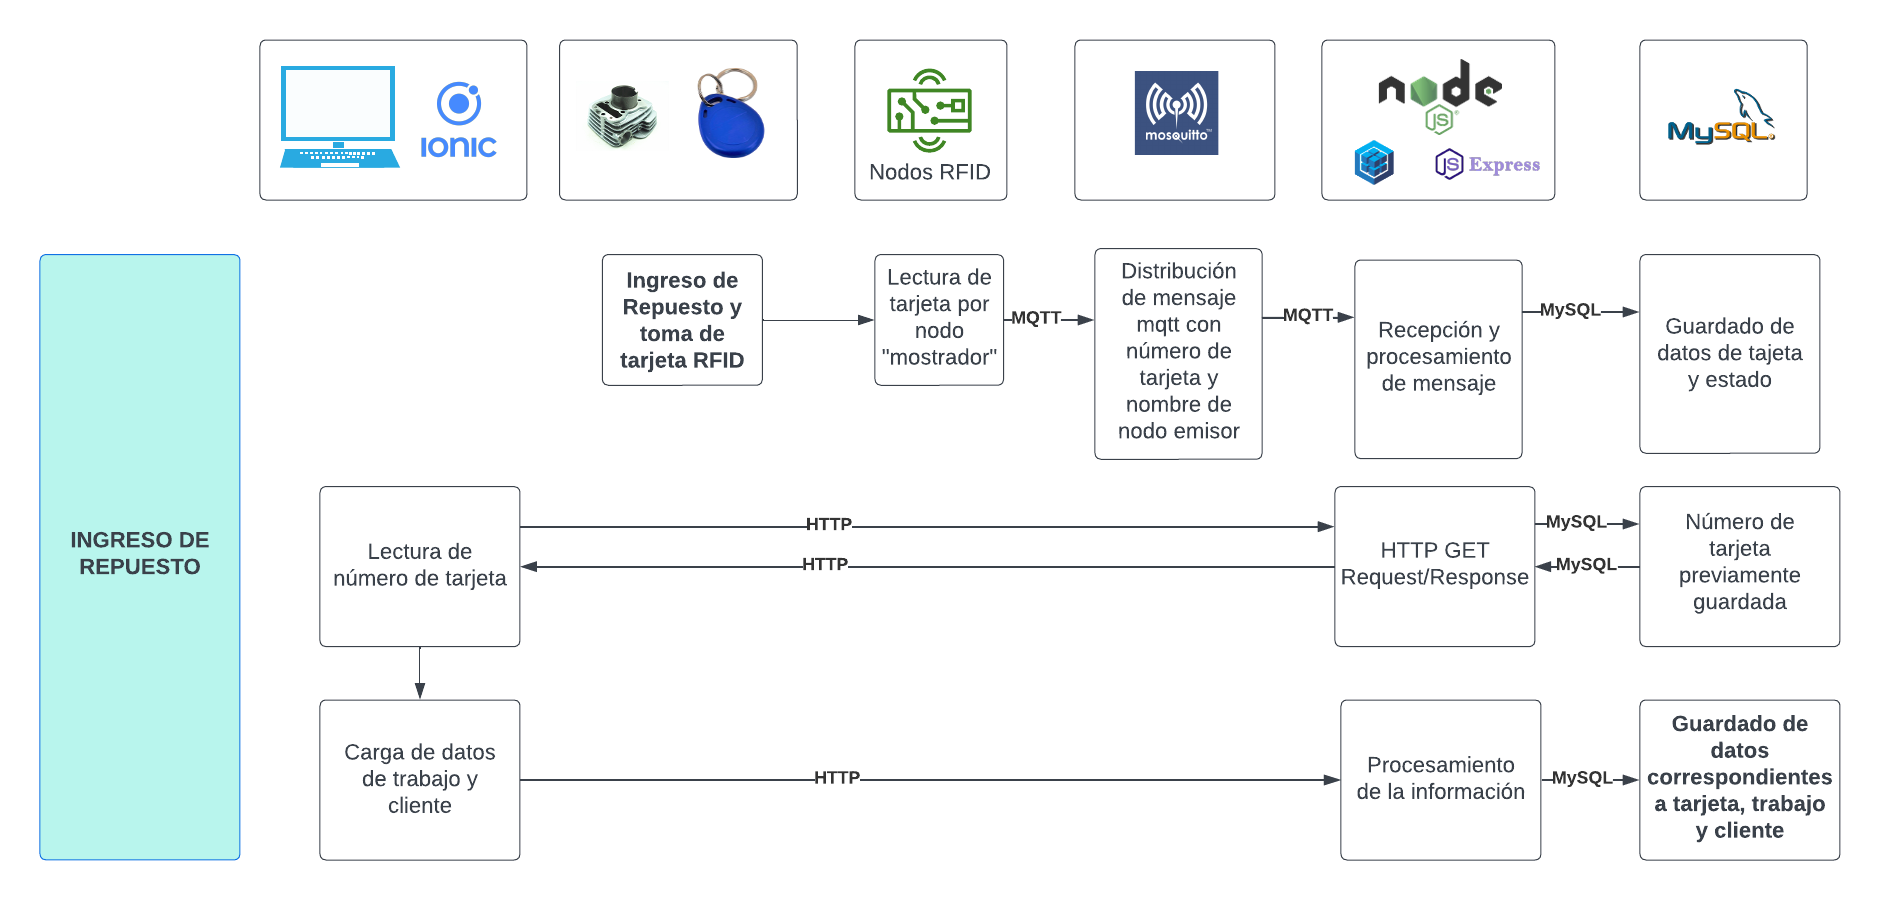
\includegraphics[scale=.20]{./Figures/flujoingreso.png}
	\caption{Flujo en el ingreso de una nueva orden de trabajo.}
	\label{fig:flujoingreso}
\end{figure}
  
El flujo comienza cuando el usuario recibe el repuesto y selecciona una tarjeta RFID libre para usarla con ese repuesto. El usuario pasa la tarjeta por el nodo ubicado en la recepción y de esta manera se registra el número de tarjeta para ser utilizada. Luego el usuario carga los datos en el sistema web, dónde ya está asignada la tarjeta previamente leída, confirma los datos y estos son guardados en la base de datos. La nueva orden de trabajo tiene su número de tarjeta, los datos del cliente y el estado por defecto \textit{en espera}.

\section{Arquitectura de datos}
\label{sec:arquitecturadatos}
En la presente sección se desarrollará la arquitectura en la base de datos MySQL, el diseño y la implementación de las funciones con el ORM Sequelize.

\subsection{Diagrama de base de datos}
\label{subsec:diagramabasededatos}

En la figura \ref{fig:diagramabbdd} se representa un diagrama UML de la base de datos con sus tablas y relaciones.

Para realizar el diseño de la base de datos se realizó un análisis de los requerimientos y los casos de usos o historias de usuario, a partir de esto se inició el diagrama con las tablas principales y sus relaciones, a medida que se avanzaba en el desarrollo de la API y del sistema  se fueron añadiendo nuevas tablas y relaciones segun las necesidades. 

\begin{figure}[ht]
	\centering
	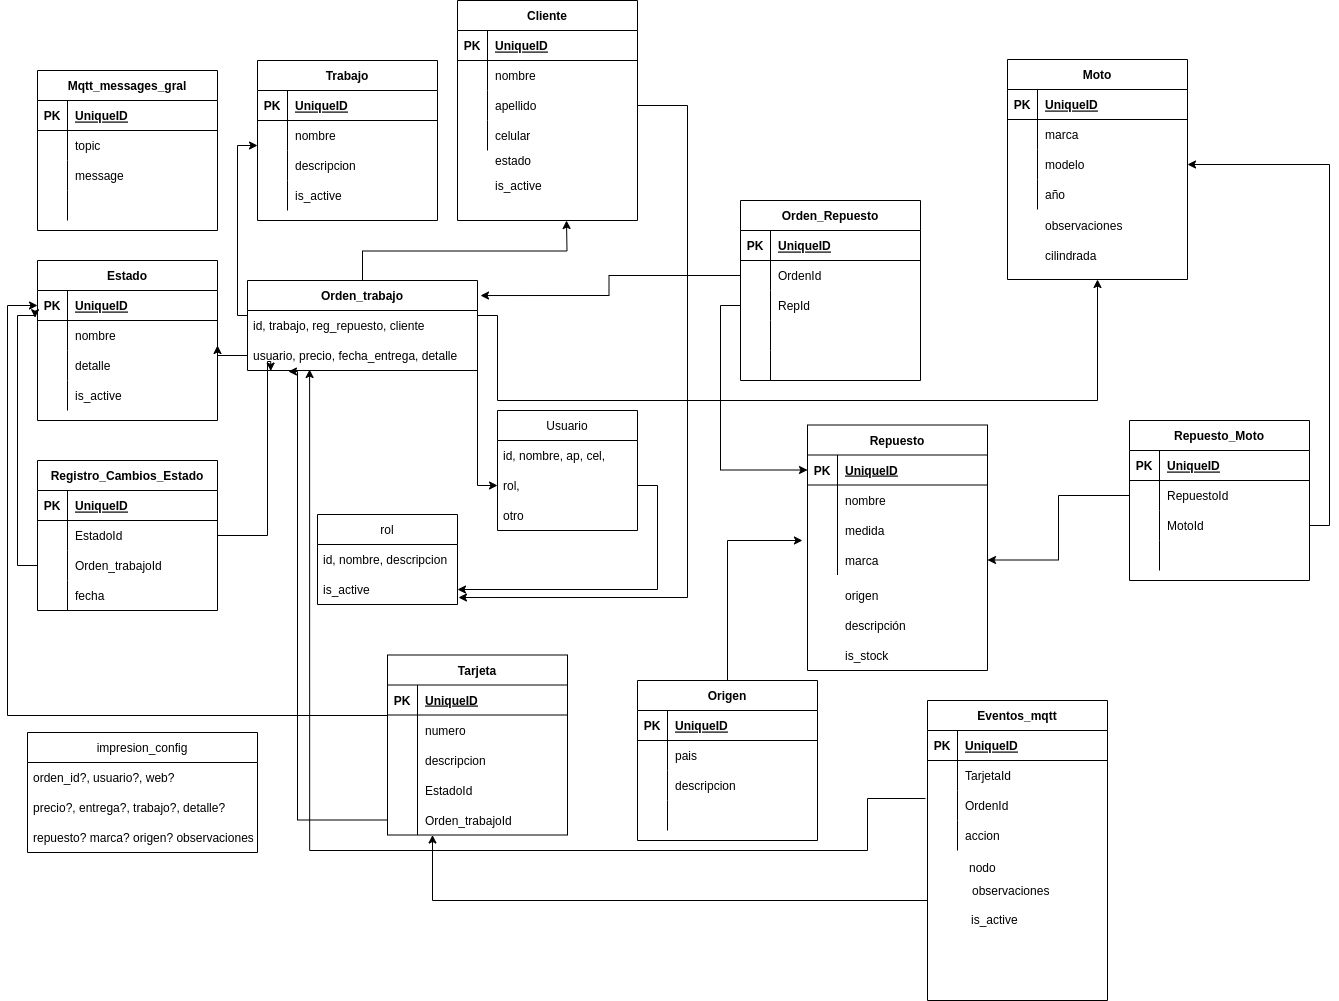
\includegraphics[scale=.25]{./Figures/diagramabbdd.png}
	\caption{Diagrama de base de datos.}
	\label{fig:diagramabbdd}
\end{figure}

\subsection{Desarrollo de modelos y tablas}
\label{subsec:modelobasededatos}

Para el desarrollo de la base de datos se utilizó el ORM Sequelize. Como se menciona en el capítulo \ref{subsec:sequelize}, existen multiples ventajas al utilizar un ORM como Sequelize en vez de directamente programar la base de datos en lenguaje SQL, se tuvieron en cuenta esas ventajas a la hora de optar por realizar el desarrollo con este ORM. 

A continuación se presentan algunos fragmentos de código fuente empleados para el desarrollo de la base de datos, siguiendo esta misma modalidad se realizaron todas las tablas de la base de datos, sus modificaciones y sus respectivas migraciones.


El siguiente código se ejecuta en la terminal de linux para crear el archivo para el modelo y el archivo para la migración de la tabla para ``Orden de trabajo". En el código se define el nombre del modelo y un atributo id. 

\begin{lstlisting}[label=cod:sequelizeclimodel,caption=Código CLI para crear modelo y migración en Sequelize.]
npx sequelize-cli model:generate --name mqtt_messages_gral --attributes id:integer
\end{lstlisting}

El siguiente código se emplea para definir el modelo completo de la tabla:

\begin{lstlisting}[caption= Código para un modelo en Sequelize.]
'use strict';
const {Model} = require('sequelize');
module.exports = (sequelize, DataTypes) => {
  class OrdenTrabajo extends Model {
    
    static associate(models) {
      //OrdenTrabajo.X pertenece a X
      OrdenTrabajo.belongsTo(models.Trabajo)
      OrdenTrabajo.belongsTo(models.Estado)
      OrdenTrabajo.belongsTo(models.Cliente)
      OrdenTrabajo.belongsTo(models.Usuario)
      OrdenTrabajo.belongsTo(models.Moto)

      //OrdenTrabajo tiene ids en la tabla Eventos_mqtt
      OrdenTrabajo.hasMany(models.Eventos_mqtt);

      //OrdenTrabajo tiene id en la tabla Tarjeta
      OrdenTrabajo.hasMany(models.Tarjeta);

      // Orden_trabjo tiene muchos Cambios de Estado N:M
      OrdenTrabajo.belongsToMany(models.Estado, {
        through: 'Registo_cambios_estado'
      })

      // Orden de trabajo tiene muchos Repuestos N:M
      OrdenTrabajo.belongsToMany(models.Repuesto, {
        through: 'Orden_Repuesto'
      })


    }
  }
  OrdenTrabajo.init({
    id: {
      allowNull: false,
      autoIncrement: true,
      primaryKey: true,
      type: DataTypes.INTEGER
    },
    precio:{
      type: DataTypes.INTEGER
    },
    entrega:{
      type: DataTypes.INTEGER
    },
    fecha_entrega_estimada:{
      type: DataTypes.DATE
    },
    detalle:{
      type: DataTypes.TEXT('long')
    },
    tarjeta:{
      type: DataTypes.STRING
    },
    ordenPapel:{
      type: DataTypes.STRING
    },
    informado:{
      type: DataTypes.BOOLEAN
    },
    is_active: {
      type: DataTypes.BOOLEAN
    },
    createdAt: {
      allowNull: false,
      type: DataTypes.DATE
    },
    updatedAt: {
      allowNull: false,
      type: DataTypes.DATE
    }
  }, {
    sequelize,
    modelName: 'OrdenTrabajo',
    tableName: 'OrdenTrabajo',
  });
  return OrdenTrabajo;
};

\end{lstlisting}

En las lineas 1 a la 4 se realizan las declaraciones de la librería y el nombre del modelo, 
luego en las lineas 6 a la 31 se definen las relaciones que tendrá el modelo, los tipos de relaciones pueden ser 1 a 1, 1 a muchos o muchos a muchos. Luego a partir de la lines 33 se definen los campos de la tabla o modelo, se definen también los atributos de los campos y el tipo de datos. En las lineas 74 y 75 se define el nombre personalizado que tendrá la tabla en la base de datos y el nombre del modelo que reconocerá el ORM. Por último en la linea 77 se retorna la Clase creada, de esta manera podrá ser utilizada en otras partes del código fuente.


\subsection{Desarrollo de migraciones}
\label{subsec:migracionesbasededatos}

Como se menciona en la sección anterior, el archivo con la estructura inicial de migraciones se crea a traves del CLI de Sequelize al momento de crear el modelo para una tabla, luego hay que personalizar esta estructura para que quede igual al modelo definido previamente. 

A continuación se representa el código \textit{javascript} para la migración del modelo ``Orden de trabajo":

\begin{lstlisting}[caption= Código para migración en Sequelize.]
'use strict';
module.exports = {
  async up(queryInterface, Sequelize) {
    await queryInterface.createTable('OrdenTrabajo', {
      id: {
        allowNull: false,
        autoIncrement: true,
        primaryKey: true,
        type: Sequelize.INTEGER
      },
      nombre: {
        type: Sequelize.STRING
      },
      precio:{
        type: Sequelize.INTEGER
      },
      entrega:{
        type: Sequelize.INTEGER
      },
      fecha_entrega_estimada:{
        type: Sequelize.DATE
      },
      detalle:{
        type: Sequelize.TEXT('long')
      },
      tarjeta:{
        type: Sequelize.STRING
      },
      ordenPapel:{
        type: Sequelize.STRING
      },
      informado:{
        type: Sequelize.BOOLEAN,
        defaultValue:false
      },
      TrabajoId:{
        type: Sequelize.INTEGER,
        references:{model:'Trabajo', key:'id'}
      },
      EstadoId:{
        type: Sequelize.INTEGER,
        references:{model:'Estado', key:'id'}
      },
      ClienteId:{
        type: Sequelize.INTEGER,
        references:{model:'Cliente', key:'id'}
      },
      
      UsuarioId:{
        type: Sequelize.INTEGER,
        references:{model:'Usuario', key:'id'}
      },
      MotoId:{
        type: Sequelize.INTEGER,
        references:{model:'Moto', key:'id'}
      },
      is_active: {
        type: Sequelize.BOOLEAN,
        defaultValue: true,
      },
      createdAt: {
        allowNull: false,
        type: Sequelize.DATE
      },
      updatedAt: {
        allowNull: false,
        type: Sequelize.DATE
      }
    });
  },
  async down(queryInterface, Sequelize) {
    await queryInterface.dropTable('OrdenTrabajo');
  }
};
\end{lstlisting}

Como se puede notar, el código es muy parecido al del modelo, con la diferencia que en este caso, ademas de los campos y sus atributos, sólo se deben definir directamente las claves que representan a las relaciones 1 a muchos que tendrá esta tabla, dejando de lado el resto de relaciones. 

Otra de las particularidades principales del archivo de migración es que contiene dos funciones que se ejecutan de manera asíncrona, la función up y down, la primera creará la tabla y la segunda se ejecuta en caso de alguna falla y elimina la tabla. 
  

\subsection{Interacción con la base de datos}
\label{subsec:interaccionbasededatos}

En Sequelize se pueden realizar todas las funciones necesarias para interactuar con la base de datos, ya sea para insertar, actualizar o eliminar registros, como así también los métodos para leer registros utilizando filtros o condiciones particulares.

A continuación se representan a modo de ejemplo algunos fragmentos de código \textit{javascript} empleados para tal fin:

Código para traer todas las órdenes de trabajo existentes, incluyendo otros modelos relacionados a este:

\begin{lstlisting}[caption= Código para traer datos en Sequelize.]
/**
 * 
 * @method getOrdenesTrabajo 
 * @description
 * Traer todas las ordenes de trabajo existentes
 * @returns
 * listado de todas las ordenes de trabajos existentes
 */
const getOrdenesTrabajo = async (req, res)=>{
    const ordenesTrabajo = await OrdenTrabajo.findAll({
        include:[
            {model:Cliente},
            {model: Estado},
            {model: Moto},
            {model: Trabajo},
            {model: Usuario},
        ]
    });
    return res.json(ordenesTrabajo)
}
\end{lstlisting}

En el siguiente código se representa de manera resumida cómo crear un nuevo registro, se quitaron algunas partes del código que son relevantes a esta sección:

\begin{lstlisting}[label=cod:nuevoregistro,caption=Código resumido para crear nuevo registro en la base de datos.]
/**
 * Crear nueva orden de trabajo
 */
const nuevaOrdenTrabajo = async (req,res) => {
        const nuevaOrdenTrabajo = await OrdenTrabajo.create(
            req.body, 
            );
  

        return res.json(nuevaOrdenTrabajo);
        
    } catch (error) {
        return res.status(400).json({
            error:error.message, 
            message:'Error cargando orden',
            context: 'api > controllers > ordenTrabajoController > nuevaOrdenTrabajo'
        })  
    }
    
}
\end{lstlisting}

En las lineas 5 y 6 es dónde se realiza la creación del registro, pasándole los datos que se reciben como parámetros en el \textit{body} de la petición HTTP.

Por último se muestra cómo actualizar un registro de la base de datos, previamente trayendo el objeto por su id:

\begin{lstlisting}[label=cod:updateregistro,caption=Código resumido para actualizar un registro en la base de datos.]

// Traigo la Orden de trabajo
let orden = await OrdenTrabajo.findOne({
            where: {
                id:req.params.id_orden,
                }
            });
            
// Modifico estado, precio, detalle y entrega de la Orden
        await orden.update(
            {
                EstadoId : estado.id,
                precio: req.body.precio,
                entrega: req.body.entrega,
                detalle: req.body.detalle
            });
\end{lstlisting}

Podemos observar que en la linea 3 se busca el registro mediante su id y se guarda el mismo en una variable, luego se utiliza esa variable para realizar la actualización de los datos, por lo que esa variable pasa a ser un ``objeto de Sequelize" que puede ser tratado directamente como entidad única de la base de datos, facilitando su uso mediante el ORM.


\section{Arquitectura backend}
\label{sec:arquitecturabackend}

\subsection{API REST}
\label{subsec:apirest}
La lógica del backend se centra principalmente en la API REST desarrollada, en la misma se utilizaron diferentes tecnologías cada una para un fin específico.
Sequelize para la conexion, desarrollo e interacción con la base de datos
Express JS para el ruteo
Javascript para la lógica
Node.Js como framework principal

% La idea de esta sección es resaltar los problemas encontrados, los criterios utilizados y la justificación de las decisiones que se hayan tomado.

% Se puede agregar código o pseudocódigo dentro de un entorno lstlisting con el siguiente código:

% \begin{verbatim}
% \begin{lstlisting}[caption= "un epígrafe descriptivo"]
% 	las líneas de código irían aquí...
% \end{lstlisting}
% \end{verbatim}

% A modo de ejemplo:

% \begin{lstlisting}[label=cod:vControl,caption=Pseudocódigo del lazo principal de control.]  % Start your code-block

% #define MAX_SENSOR_NUMBER 3
% #define MAX_ALARM_NUMBER  6
% #define MAX_ACTUATOR_NUMBER 6

% uint32_t sensorValue[MAX_SENSOR_NUMBER];		
% FunctionalState alarmControl[MAX_ALARM_NUMBER];	//ENABLE or DISABLE
% state_t alarmState[MAX_ALARM_NUMBER];						//ON or OFF
% state_t actuatorState[MAX_ACTUATOR_NUMBER];			//ON or OFF

% void vControl() {

% 	initGlobalVariables();
	
% 	period = 500 ms;
		
% 	while(1) {

% 		ticks = xTaskGetTickCount();
		
% 		updateSensors();
		
% 		updateAlarms();
		
% 		controlActuators();
		
% 		vTaskDelayUntil(&ticks, period);
% 	}
% }
% \end{lstlisting}



